%% E&G Quaternary Science Journal (EGQSJ) — Copernicus format
%% Reformatted from submission_v1.0.tex

\documentclass[egqsj, manuscript]{copernicus}

\begin{document}

\title{Multi-Site Calibration of Volcanic Sedimentation Rates and Implications for Archaeological Visibility in Java, Indonesia}

\Author[1][amien@ubhinus.ac.id]{Mukhlis}{Amien}
\Author[1]{Go Frendi}{Gunawan}

\affil[1]{Lab Data Sains, Universitas Bhinneka Nusantara, Malang, Indonesia}

\runningtitle{Volcanic sedimentation rates and archaeological visibility in Java}

\runningauthor{Amien and Gunawan}

\received{}
\pubdiscuss{}
\revised{}
\accepted{}
\published{}

\firstpage{1}

\maketitle

\begin{abstract}
Java hosts 45 active volcanoes in 129,000~km\textsuperscript{2}. Its early archaeological record is strikingly thin compared to volcanic-free regions of the same archipelago. The standard explanation is developmental: Javanese kingdoms simply came later. The explanation advanced here is geophysical: the evidence is buried.

In 1803, a Dutch colonial administrator named Nicolaus Engelhard documented two enormous stone guardian statues at the ruins of Candi Singosari in East Java---each 370~cm tall, carved from monolithic andesite in 1268~CE---with roughly half their bodies below ground. Nobody had buried them deliberately. Gunung Kelud had erupted approximately twenty times in the interval; the landscape had risen around them at \textasciitilde3.5~mm per year. Structures built of wood, brick, and thatch left no comparable marker above the sediment.

This paper calibrates what that rate means for the archaeological record as a whole. Using four sites with independently documented construction dates and measured burial depths, spanning two volcanic systems (Kelud and Merapi) and roughly 350~km of Java, we establish a mean sedimentation rate of $4.4 \pm 1.2$~mm/yr. The consistency across sites is the central finding: burial is not a local anomaly but appears to operate at a regional scale across Java's volcanic terrain. At this rate, archaeological remains from the Kanjuruhan period (\textasciitilde760~CE) now lie at 4.0--7.8~m depth in the Malang basin---beyond the reach of surface survey and at the upper limit of ground-penetrating radar. Indonesia's oldest conventionally recognized kingdom, Kutai (\textasciitilde400~CE), was found near the present ground surface in volcanic-free Kalimantan; at Javanese sedimentation rates, equivalent remains would lie beneath 7--10~m of volcanic overburden. Spatial analysis of 666 East Java sites confirms the pattern: the observable record maps survey effort and monument durability, not historical settlement intensity. We identify priority zones where high terrain suitability coincides with deep predicted burial, providing a targeting framework for future subsurface investigation.
\end{abstract}


\introduction

In 1803, a Dutch colonial administrator named Nicolaus Engelhard encountered something at the ruins of Candi Singosari that has not received the theoretical attention it deserves. Two enormous stone guardian statues---\textit{Dwarapala}, each 370~cm tall and carved from a single block of andesite---stood with roughly half their bodies below the ground. They had been installed in 1268~CE, during the reign of King Kertanegara of the Singosari kingdom \citep{kinney2003}. Nobody had buried them. The ground had risen around them at approximately 3.5~mm per year, driven by 535 years of repeated eruptions from Gunung Kelud, 35~km to the east. Only their scale made them visible at all.

Hindu-Buddhist kingdoms flourished on Java from at least the 4th century~CE, yet the material record of early Javanese polities is strikingly sparse compared to contemporaneous societies elsewhere in Southeast Asia. The kingdom of Kutai Martadipura in Kalimantan---conventionally regarded as Indonesia's oldest polity (\textasciitilde400~CE)---is known from inscribed stone pillars found near the modern ground surface in a region with zero active volcanoes \citep{vogel1918,coedes1968}. The argument of this paper is direct: the oldest Indonesian kingdom is the most \textit{visible} one. At the sedimentation rate established here, a Javanese inscription of the same age as Kutai's Yupa pillars now lies beneath approximately 7~m of volcanic overburden---invisible to surface survey, beyond the reach of conventional ground-penetrating radar. The apparent chronological primacy of non-volcanic Kalimantan over volcanic Java reflects differential preservation, not differential history.

The mechanism at work is not the catastrophic burial familiar from Pompeii, Akrotiri, or Cer\'{e}n---single eruptions sealing settlements in hours \citep{sigurdsson1985,doumas1983,sheets1992}. It is \textit{cumulative} sedimentation: repeated small eruptions depositing millimeters per event, accumulating to meters over centuries (Sect.~2.3). In Java, no point lies more than approximately 27~km from an active vent \citep{vanbemmelen1949}; there is no escape from this process, only variation in its rate. The Dwarapala statues provide direct photographic documentation at a known, measurable rate (Fig.~\ref{fig:dwarapala_photos}).

\begin{figure*}[t]
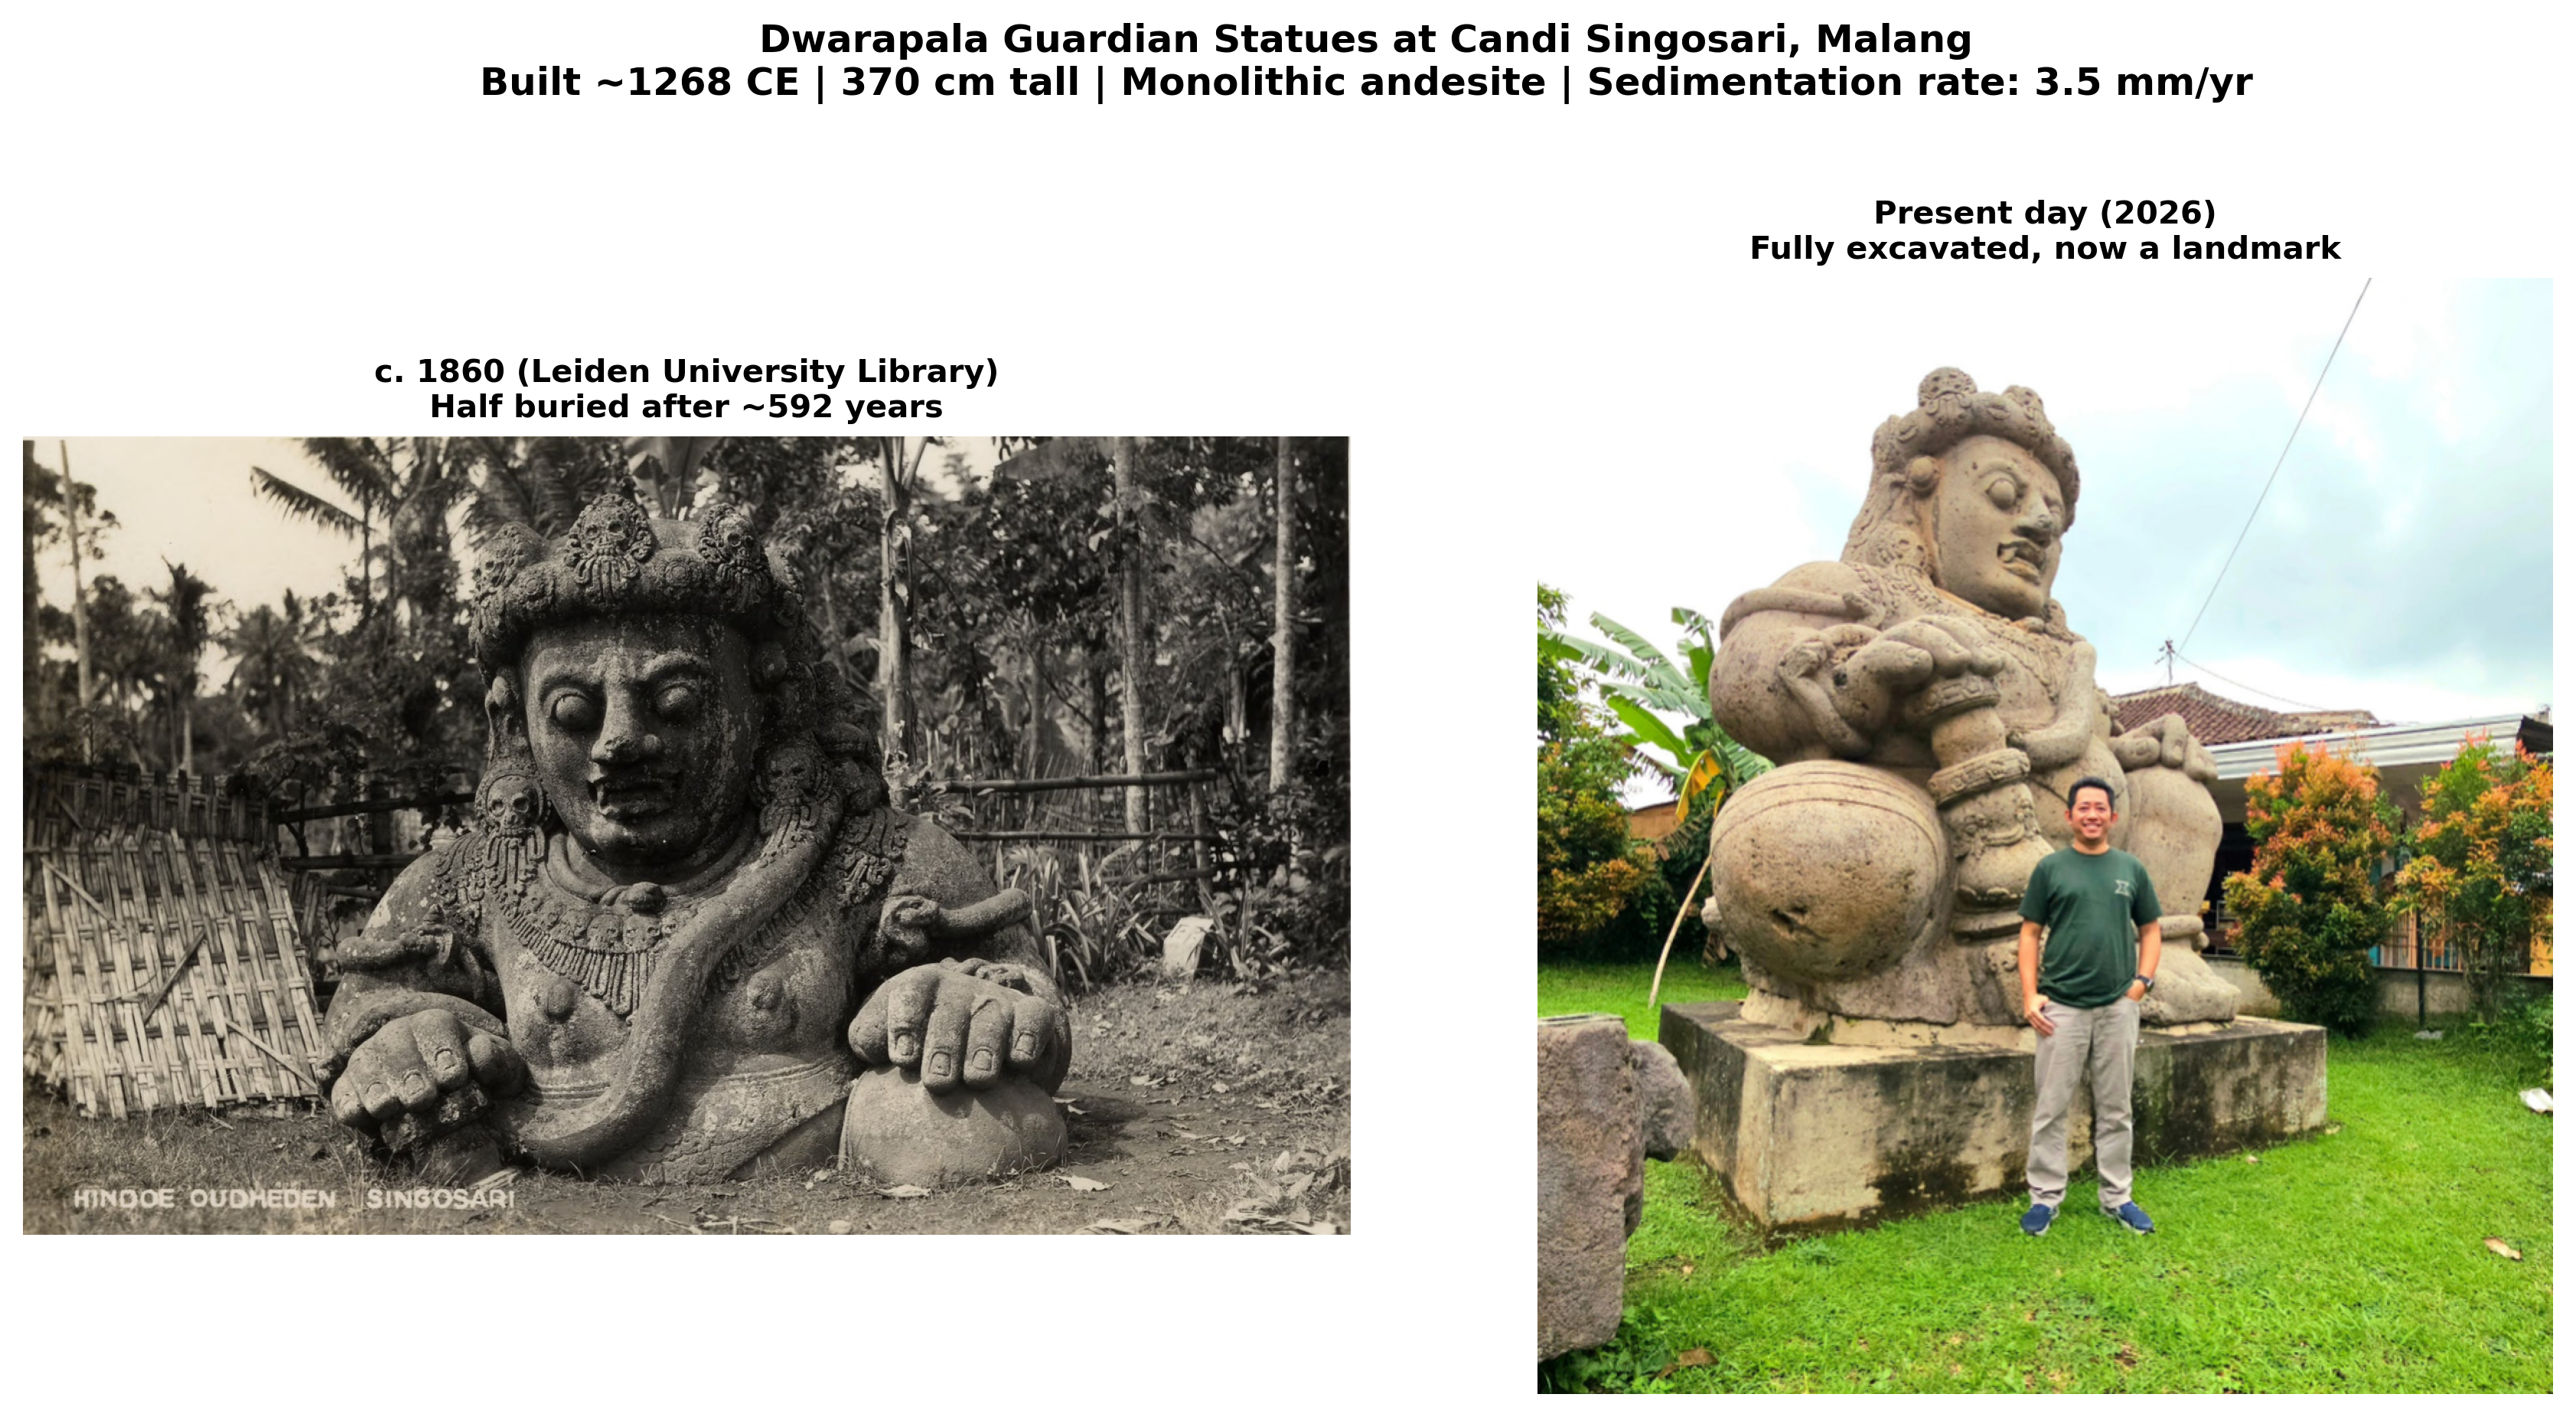
\includegraphics[width=12cm]{figures/fig0_dwarapala_comparison.png}
\caption{Dwarapala guardian statues at Candi Singosari, Malang, East Java. Left: colonial-era photograph (c.~1860) from the Leiden University Library archives, showing the statue partially buried beneath volcanic sediment---only the head, shoulders, and hands remain visible above the accumulated overburden. Right: present-day condition after excavation, revealing the full 370~cm height. The statues were constructed \textasciitilde1268~CE during the reign of Kertanegara; approximately 185~cm of volcanic overburden accumulated by their rediscovery in 1803~CE, yielding a calibrated sedimentation rate of 3.5~mm/yr (Sect.~3.2).}
\label{fig:dwarapala_photos}
\end{figure*}

Surface visibility is a recognized problem in archaeological survey \citep{wandsnider1992,french2003}, but its implications for volcanic landscapes in island Southeast Asia have been largely ignored. Research here has focused on monumental stone architecture---the class of evidence most resistant to burial \citep{degroot2009}---and the circularity is plain: we find stone temples because they protrude through sediment; we interpret their distribution as reflecting settlement patterns; and we overlook the wooden settlements that constituted the overwhelming majority of historical habitation.

The empirical foundation is a four-site calibration. We compiled construction dates and measured burial depths for four archaeological sites: the Dwarapala statues at Candi Singosari (\textasciitilde1268~CE, Kelud volcanic system) and three Hindu-Buddhist temples near Merapi in Central Java (Sambisari, Kedulan, and Kimpulan, all 9th century~CE). These span roughly 350~km of Java and two geologically distinct volcanic systems. Kelud has produced 37 confirmed eruptions since 1000~CE \citep{gvp2024}. Merapi is one of the world's most persistently active stratovolcanoes \citep{gertisser2012}. The sedimentation rates converge within a factor of two. That was not guaranteed, and we consider it the central result.

Those rates are applied to project burial depths for successive historical periods: Kanjuruhan-era (\textasciitilde760~CE) remains in the Malang basin are predicted to lie at 4.0--7.8~m---exceeding the reach of surface survey and approaching the upper limit of ground-penetrating radar \citep{putra2019}. A spatial analysis of 666 known archaeological sites in East Java tests the corollary: if the taphonomic argument is correct, the observable record should map survey effort and monument scale, not settlement patterns. It does. Priority zones for future subsurface investigation are identified where terrain suitability and predicted burial depth are both high.


\section{Background}

\subsection{Java as a volcanic burial zone}

Java hosts 45 active volcanoes across approximately 129,000~km\textsuperscript{2}---a volcanic density of 0.35 per 1,000~km\textsuperscript{2}, the highest of any major Indonesian island and approximately six times that of Sumatra (0.06/1,000~km\textsuperscript{2}) \citep{vanbemmelen1949}. The average spacing between volcanic centers is \textasciitilde54~km, meaning that no point on Java is more than approximately 27~km from the nearest active volcano. Since tephra from VEI~3--4 eruptions can deposit measurable ash at 50--100+~km from the source \citep{newhall1982}, the entire island lies within the depositional range of at least one---and often multiple---volcanic centers.

There is no part of Java that is not downwind of an active volcano. The relevant archaeological question is therefore not whether volcanic sedimentation occurs at a given location, but how much has accumulated since a site was occupied---a function of distance from active vents, local topography, and the eruption history of whichever volcano sits upwind. Java does not have a volcanic burial problem in some places. It has one everywhere, to varying degrees.

East Java province alone encompasses seven major active centers: Kelud, Semeru, Arjuno-Welirang, Bromo, Lamongan, Raung, and Ijen. The Brantas River basin---which hosted the Singosari (1222--1293~CE) and Majapahit (1293--\textasciitilde1500~CE) kingdoms---sits in the depositional path of Kelud (35~km east), Arjuno-Welirang (25~km north), and Semeru (60~km southeast). Kelud alone has produced 37 confirmed eruptions since 1000~CE \citep{gvp2024,maeno2019}.

In Central Java, Mount Merapi---one of the world's most active stratovolcanoes---has buried a cluster of 9th-century Hindu-Buddhist temples to depths of 3--7~m \citep{lavigne2000,thouret2000}. These buried temples (Sambisari, Kedulan, Kimpulan) were discovered accidentally during modern construction and mining activities, not through systematic archaeological survey.

\subsection{The observable archaeological record in East Java}

Our compilation of known archaeological sites in East Java (Sect.~3.1) identified 666 unique entries, of which only 391 (59\%) have usable spatial coordinates. The dataset is dominated by stone monuments (\textit{candi}) from the Singosari and Majapahit periods (13th--15th centuries~CE) \citep{kinney2003}. Earlier periods are poorly represented: pre-10th century sites constitute less than 5\% of the geocoded total.

This temporal distribution reflects two complementary pressures. Survey has historically concentrated on the Singosari-Majapahit heartland around Blitar, Malang, and Mojokerto. And older sites are more deeply buried---having accumulated more volcanic overburden---making them less likely to surface at all.

A conceivable objection is that this pre-10th century absence reflects genuine demographic scarcity rather than taphonomic loss. The objection fails quantitatively. Ethnographic carrying capacity estimates for tropical island Southeast Asian agriculture range from approximately 5 to 30 persons/km\textsuperscript{2} for swidden and early wet-rice systems \citep{bellwood2017,kirch2000,baylisssmith1980}. Applied conservatively to Java's habitable lowlands---roughly half the island's 129,000~km\textsuperscript{2}---these densities yield a pre-400~CE population of approximately 590,000--3,900,000, comparable to contemporaneous Dvaravati Thailand and considerably exceeding early Sriwijaya. At standard Austronesian village sizes of 100--200 persons, even the lower bound implies roughly 3,000 settlements of standard archaeological visibility. The observed count of pre-400~CE sites in the volcanic interior is 0--3. The gap is approximately 3,220-fold (lower-bound estimate: 5 persons/km\textsuperscript{2}, \textasciitilde50\% habitable area, 100 persons per village). Low population does not generate a 3,220-fold absence.

The inscription record provides independent confirmation of a different kind. Systematic reading of all 268 surviving Javanese inscriptions in the DHARMA epigraphic database (8th--13th centuries~CE) \citep{dharma2024} finds that 170 (63.4\%) explicitly mention organic building materials---wood (\textit{kayu}), bamboo (\textit{bambu}), palm thatch (\textit{atap}), palm fiber (\textit{ijuk})---while only 73 (27.2\%) mention stone or brick (binomial $p < 0.0001$). The people who carved these stone inscriptions lived predominantly in structures that do not survive. The archaeological blank of volcanic Java is not an absence of civilization. It is a preservation filter that passes stone and rejects wood.

\subsection{Volcanic taphonomy}

Most of what archaeologists know about volcanic burial comes from Pompeii. This is a problem. Pompeii was buried in eighteen hours; Candi Sambisari was buried over roughly a thousand years. These are not the same process, and they do not produce the same kind of archaeological evidence.

Catastrophic volcanic burial---a single eruption sealing an entire settlement in hours---is spectacular and well-studied \citep{sigurdsson1985,doumas1983,sheets1992}. It also creates conditions unusual enough to attract decades of excavation attention. \textit{Cumulative} volcanic burial, by contrast, generates no single dramatic event to excavate. Ash arrives in centimeters per eruption, lahars rework it downslope, and every decade the ground is fractionally higher than the decade before. After five centuries, a surface that was once at eye level is two meters underground. After fifteen centuries, it may be six. Nothing announces this; no emergency response is triggered; no excavation follows. The site simply becomes, gradually and completely, invisible.

\subsection{The Kutai comparison}

The oldest known kingdom in the Indonesian archipelago is Kutai Martadipura (\textasciitilde400~CE), located in East Kalimantan---a region with zero active volcanoes across 544,000~km\textsuperscript{2} \citep{vogel1918}. Its Yupa inscriptions were found near the present ground surface.

The contrast is stark: Java has 45 active volcanoes in 129,000~km\textsuperscript{2}; Kalimantan has zero in 544,000~km\textsuperscript{2}. At the mean Javanese sedimentation rate of 4.4~mm/yr, a Kutai-era (\textasciitilde400~CE) inscription in the Malang basin would now lie beneath 4--10~m of volcanic overburden---invisible to any surface survey. The same inscription in Kalimantan sits exactly where it was placed 1,600 years ago, because there is no volcanic sedimentation to bury it.

Kutai's apparent chronological primacy over Javanese polities of similar or greater antiquity may therefore reflect differential preservation conditions rather than genuine temporal precedence \citep{coedes1968,miksic2004}. The ``oldest kingdom'' is simply the most \textit{visible} one---a direct consequence of volcanic density asymmetry between islands.

\subsection{The West Java control: within-island preservation asymmetry}

A cross-island comparison between Java and Kalimantan, while suggestive, is subject to the objection that the two islands differ in many ways besides volcanism: ecology, trade routes, cultural trajectories, research history. The strongest evidence for taphonomic bias is not a cross-island comparison at all, but a within-island one.

West Java's non-volcanic coastal zone preserves a rich pre-400~CE material record that its volcanic interior entirely lacks---on the same island, during the same broad period. The Buni Cultural Complex (Tangerang coast, \textasciitilde200~BCE--500~CE) represents a dense concentration of organic-rich cultural material---pottery, glass and carnelian beads, iron tools, bronze ornaments---distributed across dozens of sites in a region of zero active volcanism \citep{wibisono1994,bellina2014}. Batujaya (Karawang regency, 2nd--5th century~CE), on the same non-volcanic coastal plain, preserves a substantial brick Buddhist complex---the oldest confirmed Buddhist architectural remains in the archipelago \citep{manguin2011}. Both complexes document demographically significant, organizationally complex societies in Java during precisely the period for which the volcanic interior offers nothing.

This within-island asymmetry is consistent with what the taphonomic framework predicts. Same island. Same broad time window. The difference is geology: non-volcanic coastal plain versus volcanic alluvial basin. A caveat is necessary: the Buni and Batujaya communities were embedded in maritime trade networks connecting the Malay Peninsula and the Indian Ocean \citep{bellina2014,manguin2011}; interior volcanic Java may have supported culturally distinct populations whose material absence reflects genuine difference rather than taphonomic loss. The comparison controls for island-level factors---climate, deep linguistic history, broad ecology---but not for the coastal-interior economic divergence that runs through much of Island Southeast Asian prehistory. We present it as suggestive, not definitive.


\section{Data and Methods}

\subsection{Archaeological site dataset}

We compiled a database of known archaeological sites in East Java province from three complementary sources. First, we queried the OpenStreetMap Overpass API for all features tagged with \texttt{historic=*} within the Jawa Timur administrative boundary (bounding box: 6.5--9.0\textdegree{}S, 111.0--115.0\textdegree{}E), yielding 281 geolocated features. Second, we queried the Wikidata SPARQL endpoint for entities with coordinate property P625 within the same bounding box, recovering 16 precisely located sites. Third, we scraped the Indonesian-language Wikipedia article ``Daftar candi di Indonesia'' for 369 additional entries.

To increase spatial coverage, we geocoded the 369 coordinate-less entries using the OpenStreetMap Nominatim API with progressive query refinement. Of 369 queries, 94 returned valid coordinates within the study area (25.5\% success rate). After spatial deduplication within a 100~m radius, the final dataset contains 666 unique site entries, of which 391 have usable coordinates (58.7\% geocoding rate). Within the East Java analytical bounds, 383 geocoded sites were used for spatial analysis.

\textbf{Limitation:} The dataset is heavily biased toward stone monuments (\textit{candi}) that survived volcanic burial due to their monumental scale. Wooden settlements, which likely constituted the vast majority of historical habitation, are systematically absent---precisely the pattern predicted by the taphonomic bias hypothesis.

\subsection{The Dwarapala calibration}

The primary empirical anchor for our burial depth framework is the pair of Dwarapala guardian statues at Candi Singosari, Malang Regency, East Java.

\textbf{Known parameters:}
\begin{itemize}
  \item Construction date: \textasciitilde1268~CE (reign of Kertanegara, Singosari Kingdom)
  \item Discovery date: 1803~CE, by Nicolaus Engelhard
  \item Physical dimensions: 370~cm seated height, \textasciitilde40 tonnes, monolithic andesite
  \item Condition at discovery: ``\textit{separuh tubuh terpendam}'' (half the body buried)
  \item Estimated burial depth: \textasciitilde185~cm
  \item Elapsed time: 1803~$-$~1268~$=$~535 years
\end{itemize}

\textbf{Calculated sedimentation rate:}
\begin{equation}
  R = \frac{185~\text{cm}}{535~\text{yr}} = 0.35~\text{cm/yr} = 3.5~\text{mm/yr}
\end{equation}

\textbf{Cross-validation:} Gunung Kelud erupted approximately 20 times between 1268 and 1803~CE. Documented VEI~3--4 eruptions deposit 2--20~cm of ash at Malang distance (\textasciitilde35~km). Twenty eruptions at an average of \textasciitilde5~cm per event would account for \textasciitilde100~cm of the 185~cm total burial. The remainder (\textasciitilde85~cm) is attributable to secondary remobilization (lahars, reworked tephra), contributions from Semeru and Arjuno-Welirang, and non-volcanic aggradation \citep{gvp2024,maeno2019}. We note that the rates reported here represent \textit{total landscape aggradation} in volcanic terrain, not pure primary tephra accumulation; for archaeological burial, however, the total rate is the operationally relevant metric regardless of depositional source.

Fig.~\ref{fig:timeline} illustrates the Dwarapala burial timeline from construction to present.

\begin{figure}[t]
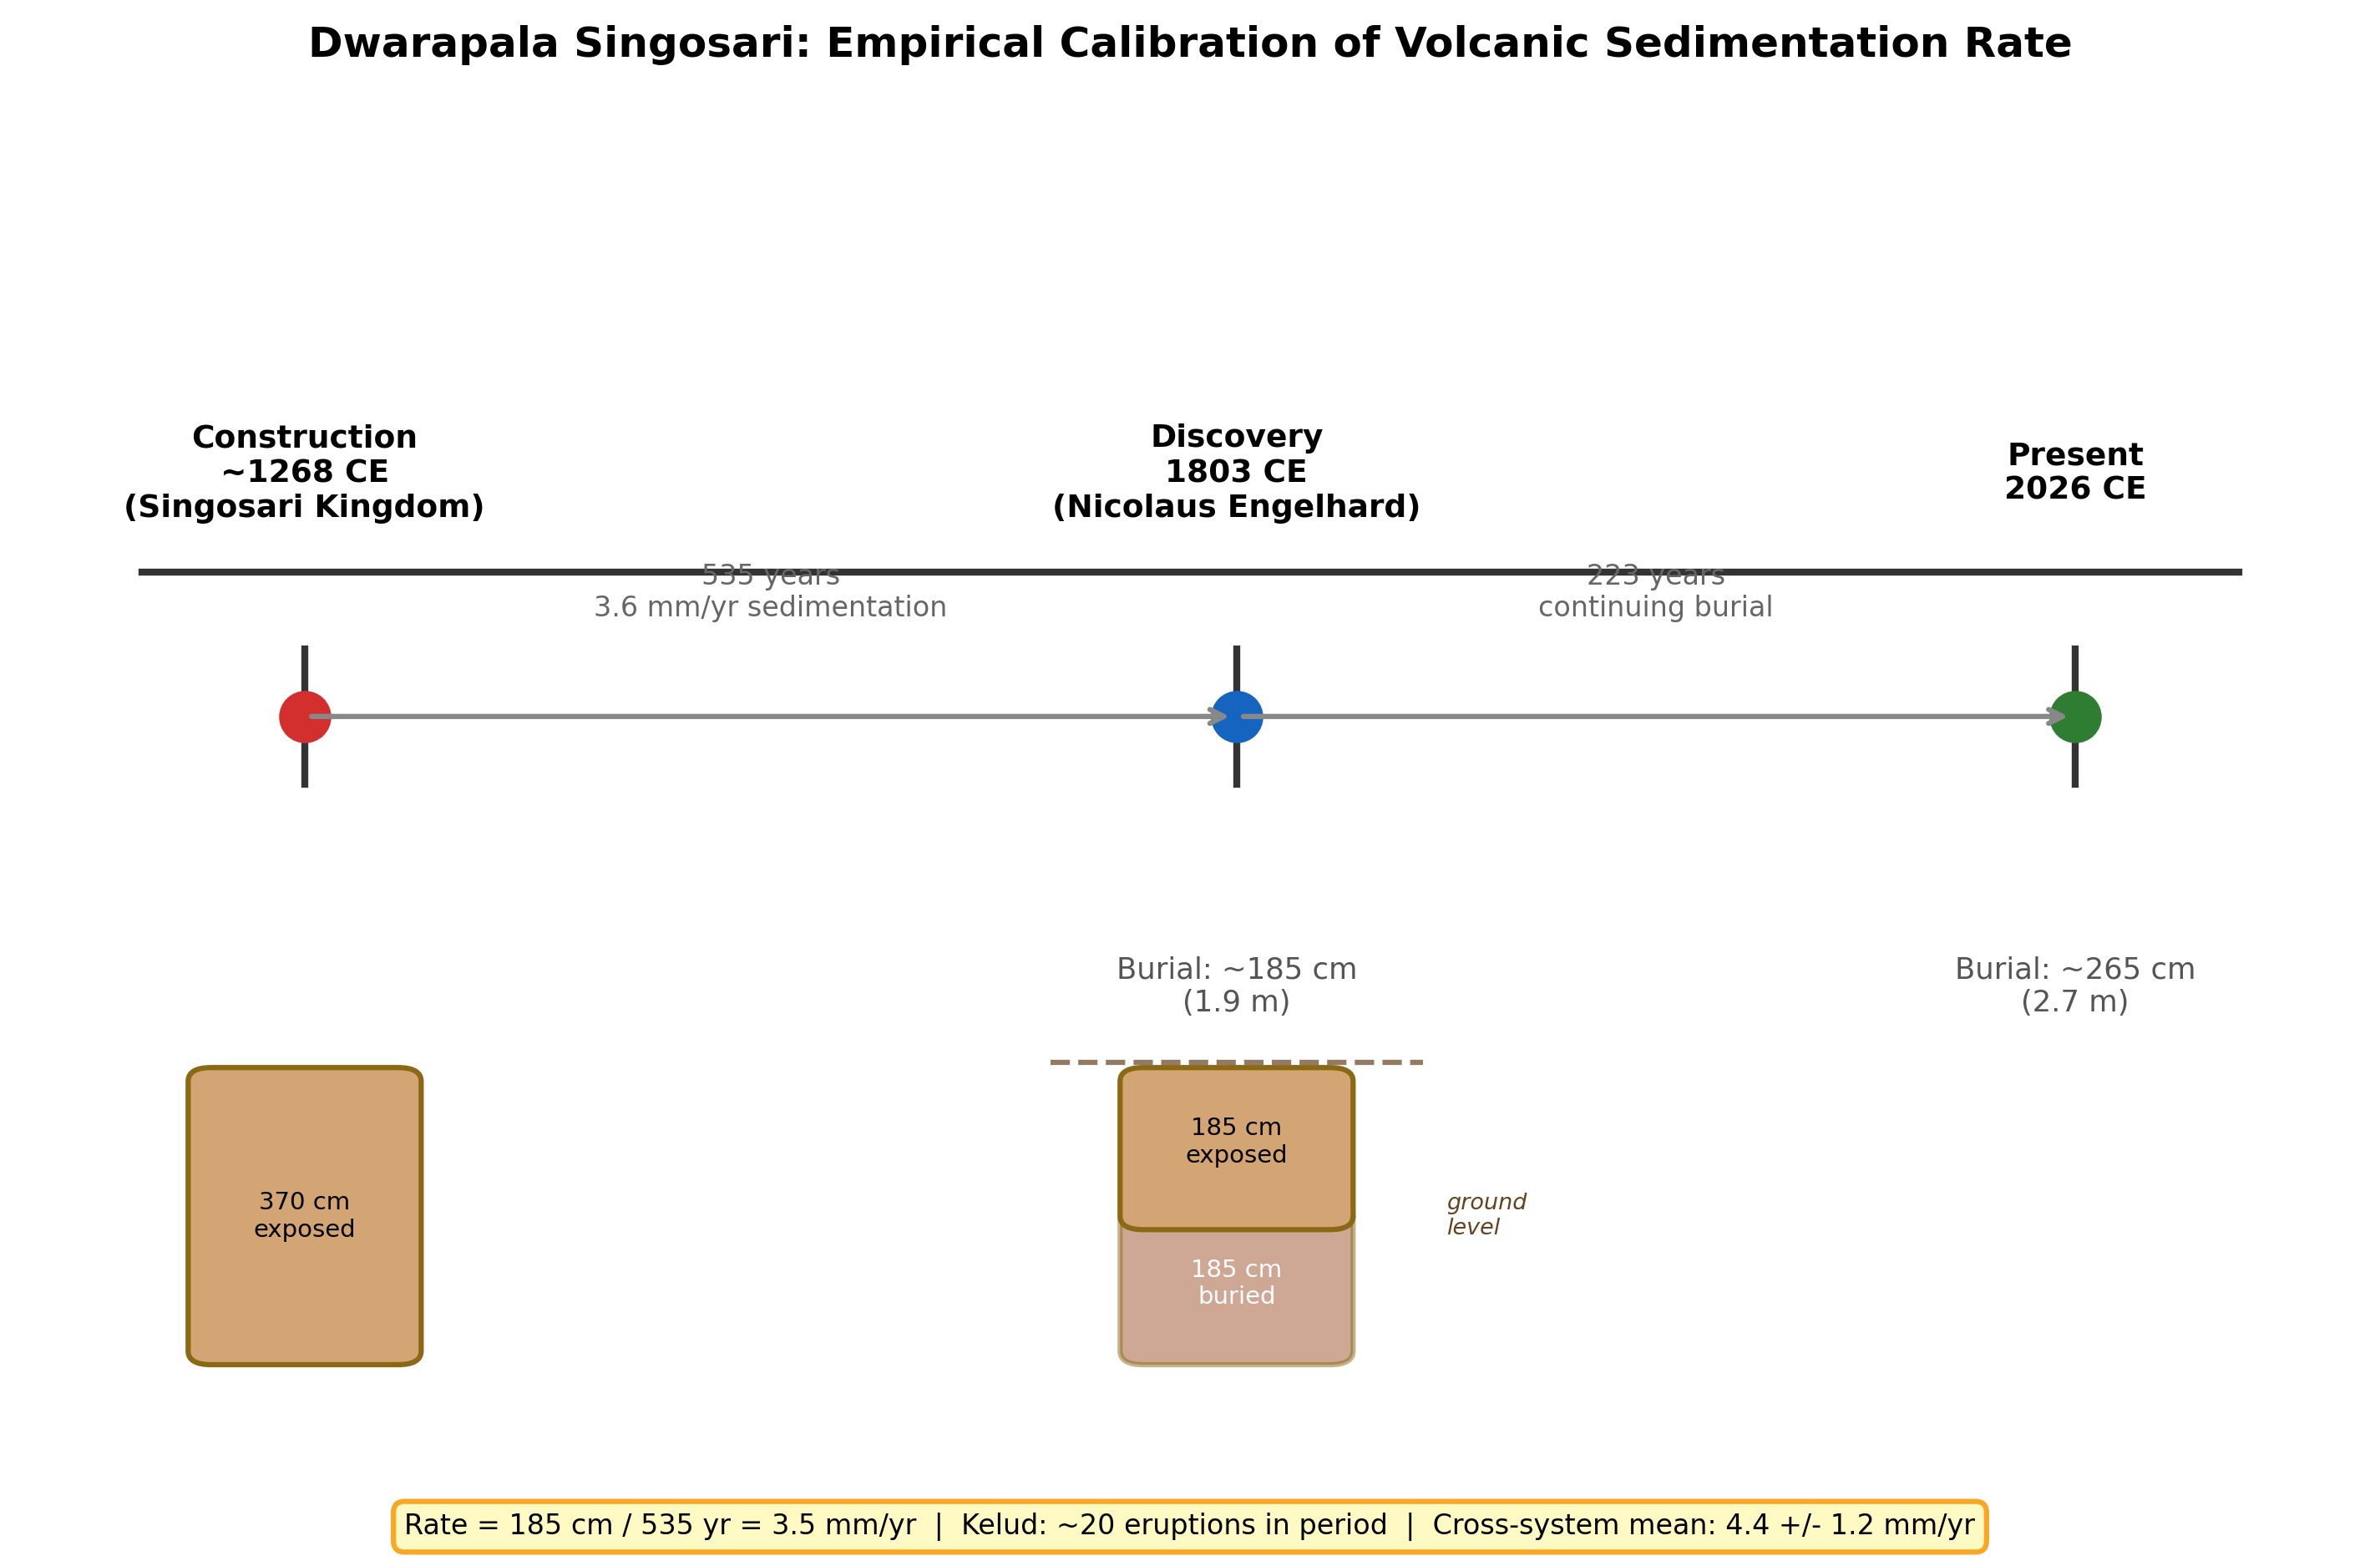
\includegraphics[width=8.3cm]{figures/fig1_dwarapala_timeline.png}
\caption{Dwarapala Singosari burial timeline. The statues were constructed \textasciitilde1268~CE at full height (370~cm) and discovered in 1803~CE with approximately half (185~cm) buried by volcanic sedimentation, yielding a cumulative rate of 3.5~mm/yr. The cross-system mean from four calibration points is $4.4 \pm 1.2$~mm/yr.}
\label{fig:timeline}
\end{figure}

\subsection{Secondary calibration points}

To assess whether the Dwarapala rate is a local anomaly or representative of a Java-wide phenomenon, we compiled three additional calibration points from Central Java's Merapi volcanic system (Table~\ref{tab:calibration}).

\begin{table}[t]
\caption{Empirical calibration points for volcanic sedimentation rates at archaeological sites in Java. BPCB-Jatim and BPCB-DIY are Indonesia's regional heritage conservation agencies (\textit{Balai Pelestarian Cagar Budaya}, Ministry of Education and Culture); burial depths are from their published excavation reports. Sambisari and Kedulan depths are cited in \citet{lavigne2000} and \citet{thouret2000}.}
\label{tab:calibration}
\begin{tabular}{lcccccc}
\tophline
Site & Built (CE) & Discovered & Depth (cm) & System & Rate (mm/yr) & Source \\
\middlehline
Dwarapala Singosari & \textasciitilde1268 & 1803 & \textasciitilde185 & Kelud & 3.5 & BPCB Jatim \\
Candi Sambisari & \textasciitilde835 & 1966 & 500--650 & Merapi & 4.4--5.7 & BPCB DIY \\
Candi Kedulan & \textasciitilde869 & 1993 & 600--700 & Merapi & 5.3--6.2 & BPCB DIY \\
Candi Kimpulan & \textasciitilde900 & 2009 & 270--500 & Merapi & 2.4--4.5 & \citet{putra2019} \\
\bottomhline
\end{tabular}
\belowtable{}
\end{table}

Across all four sites, the computed rates span 2.4--6.2~mm/yr. Taking the midpoint of each site's range (Dwarapala: 3.5; Sambisari: 5.1; Kedulan: 5.8; Kimpulan: 3.5~mm/yr) yields a mean of $4.4 \pm 1.2$~mm/yr (1$\sigma$, $n=4$). The full observed range of 2.4--6.2~mm/yr is used for all subsequent projections. The consistency across two independent volcanic systems---Kelud in East Java and Merapi in Central Java---demonstrates that mm/yr-scale burial of archaeological sites is systematic and Java-wide, not a local anomaly (Fig.~\ref{fig:rates}).

\subsection{Independent validation: eruption--site correlation dataset}

As an independent check on these calibration rates, we compiled a dataset of 51 documented eruption--archaeological site correlations from across 12 volcanic systems in Island Southeast Asia. Sources were historical and colonial-era records documenting specific volcanic events and their effects on specific known sites; 86\% of the evidence was primary (directly observed and recorded, not inferred from proximity). Of the 51 pairs, 24 include physically measured burial depths. The mean measured depth across these 24 sites is 3.41~m (median 2.50~m), consistent with our four-site calibration mean of 4.4~mm/yr applied over a 760-year horizon (expected depth: 3.3~m). This dataset shares no sites with our primary calibration and provides independent confirmation that meter-scale burial is a normal outcome of multi-century volcanic sedimentation at archaeological sites across the region.

\begin{figure}[t]
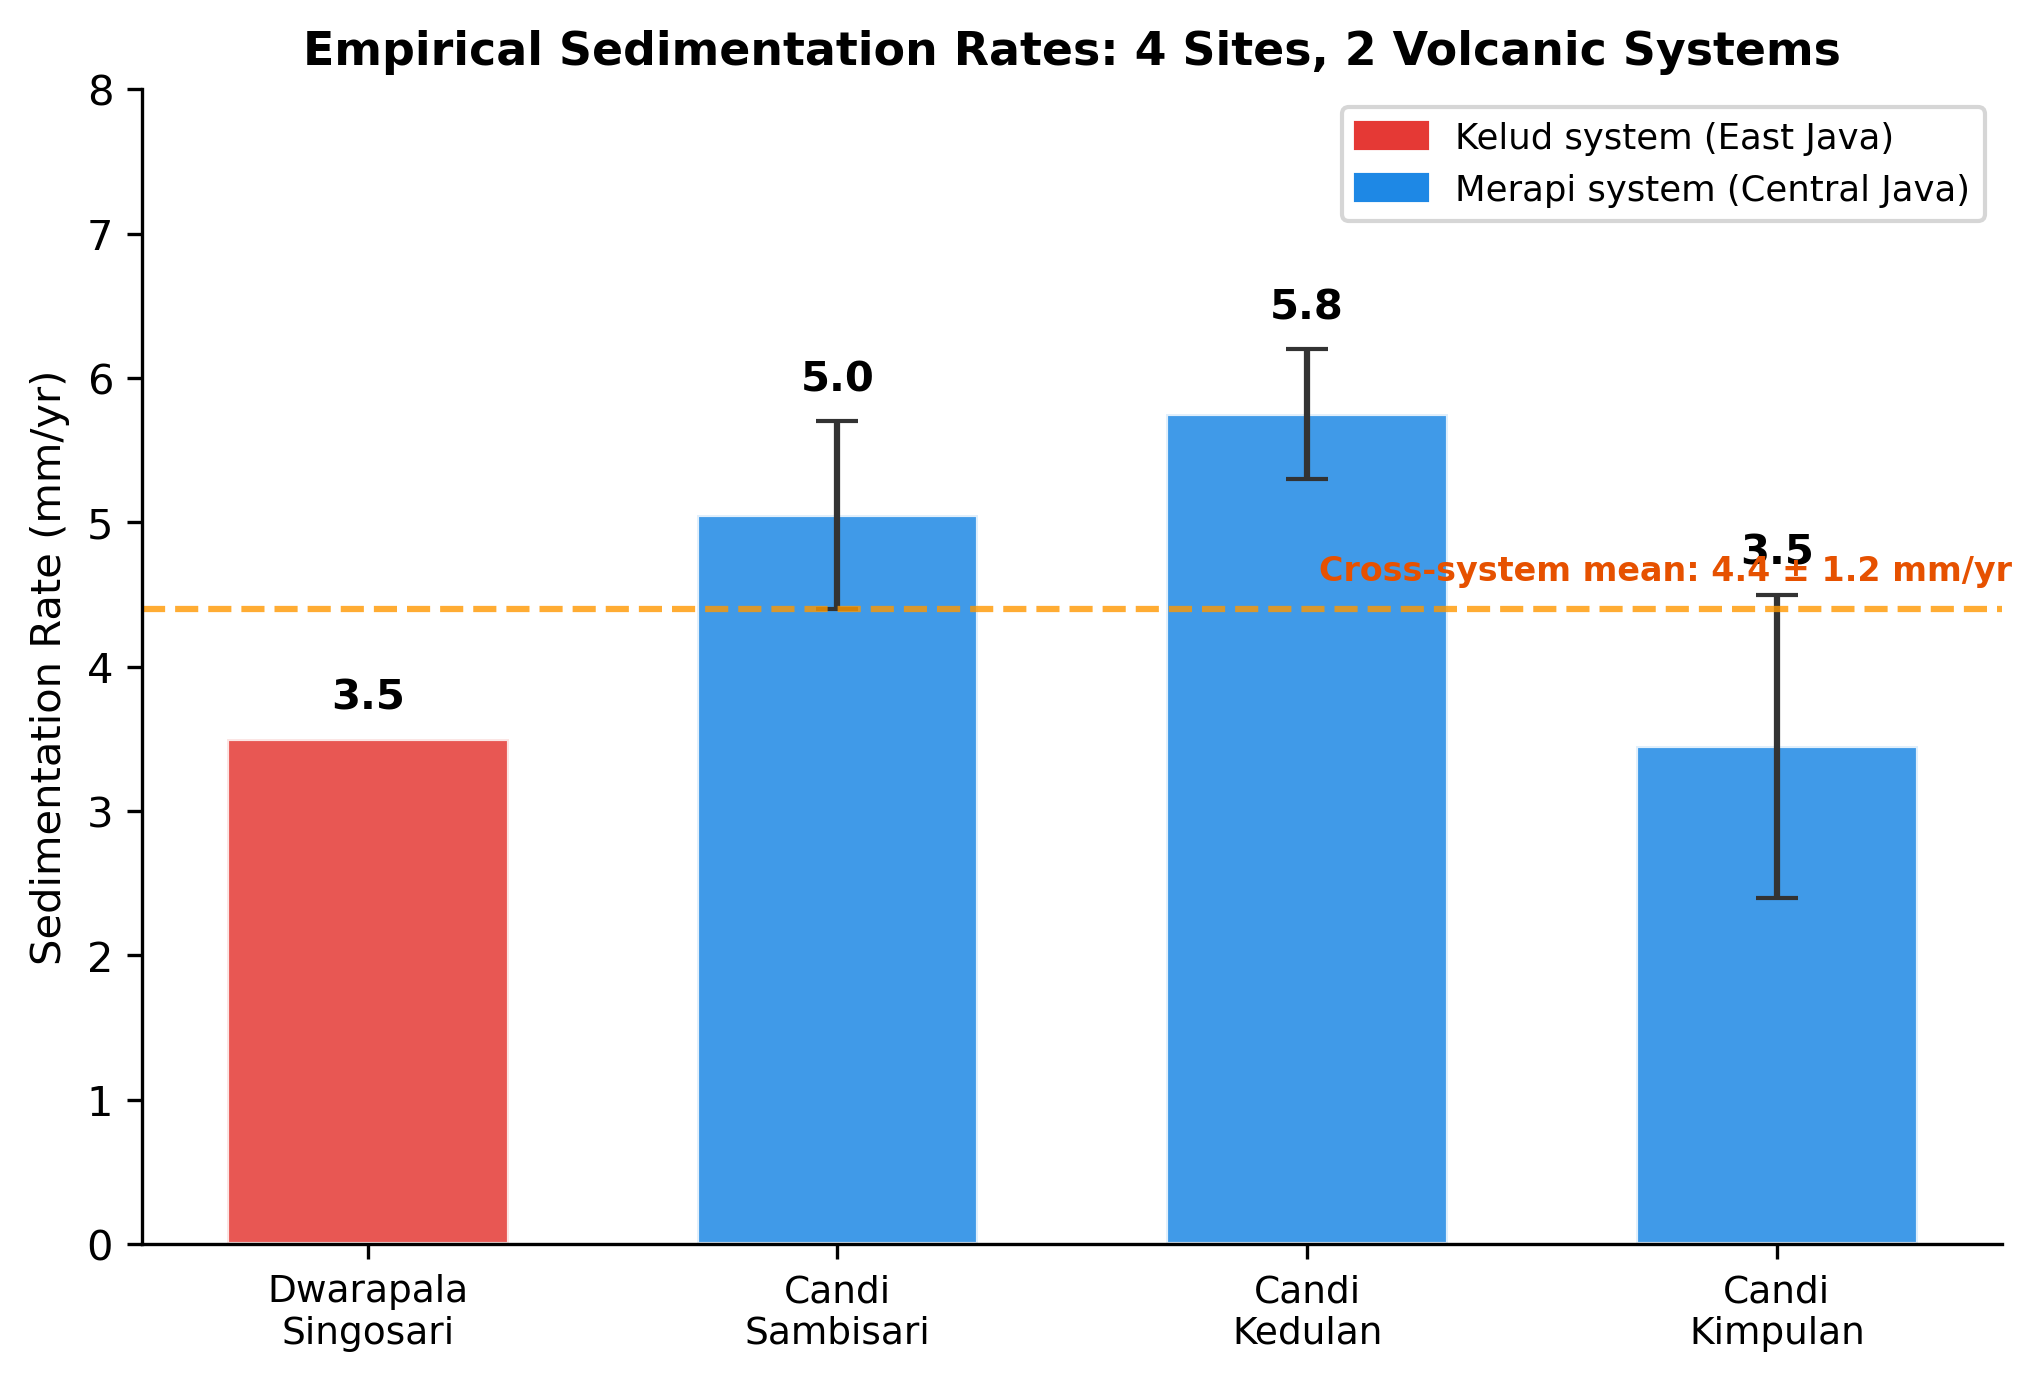
\includegraphics[width=8.3cm]{figures/fig3_calibration_rates.png}
\caption{Empirical sedimentation rates from four archaeological sites across two volcanic systems. Error bars show the range from reported depth uncertainty. The cross-system mean is $4.4 \pm 1.2$~mm/yr.}
\label{fig:rates}
\end{figure}

\subsection{Burial depth projection model}

Using the empirically-derived rate range, we estimate expected overburden depth by era:

\begin{equation}
  D(\text{era}) = R \times (T_{\text{present}} - T_{\text{era}})
\end{equation}

where $R$ ranges from 2.4 to 6.2~mm/yr and $T_{\text{present}} = 2026$~CE. This linear model is a first-order approximation; actual deposition is episodic, with eruption clusters interspersed by quiescent periods and subject to compaction. The wide rate range (2.4--6.2~mm/yr) partially captures this variability. Results are presented in Fig.~\ref{fig:depth}.

\begin{figure*}[t]
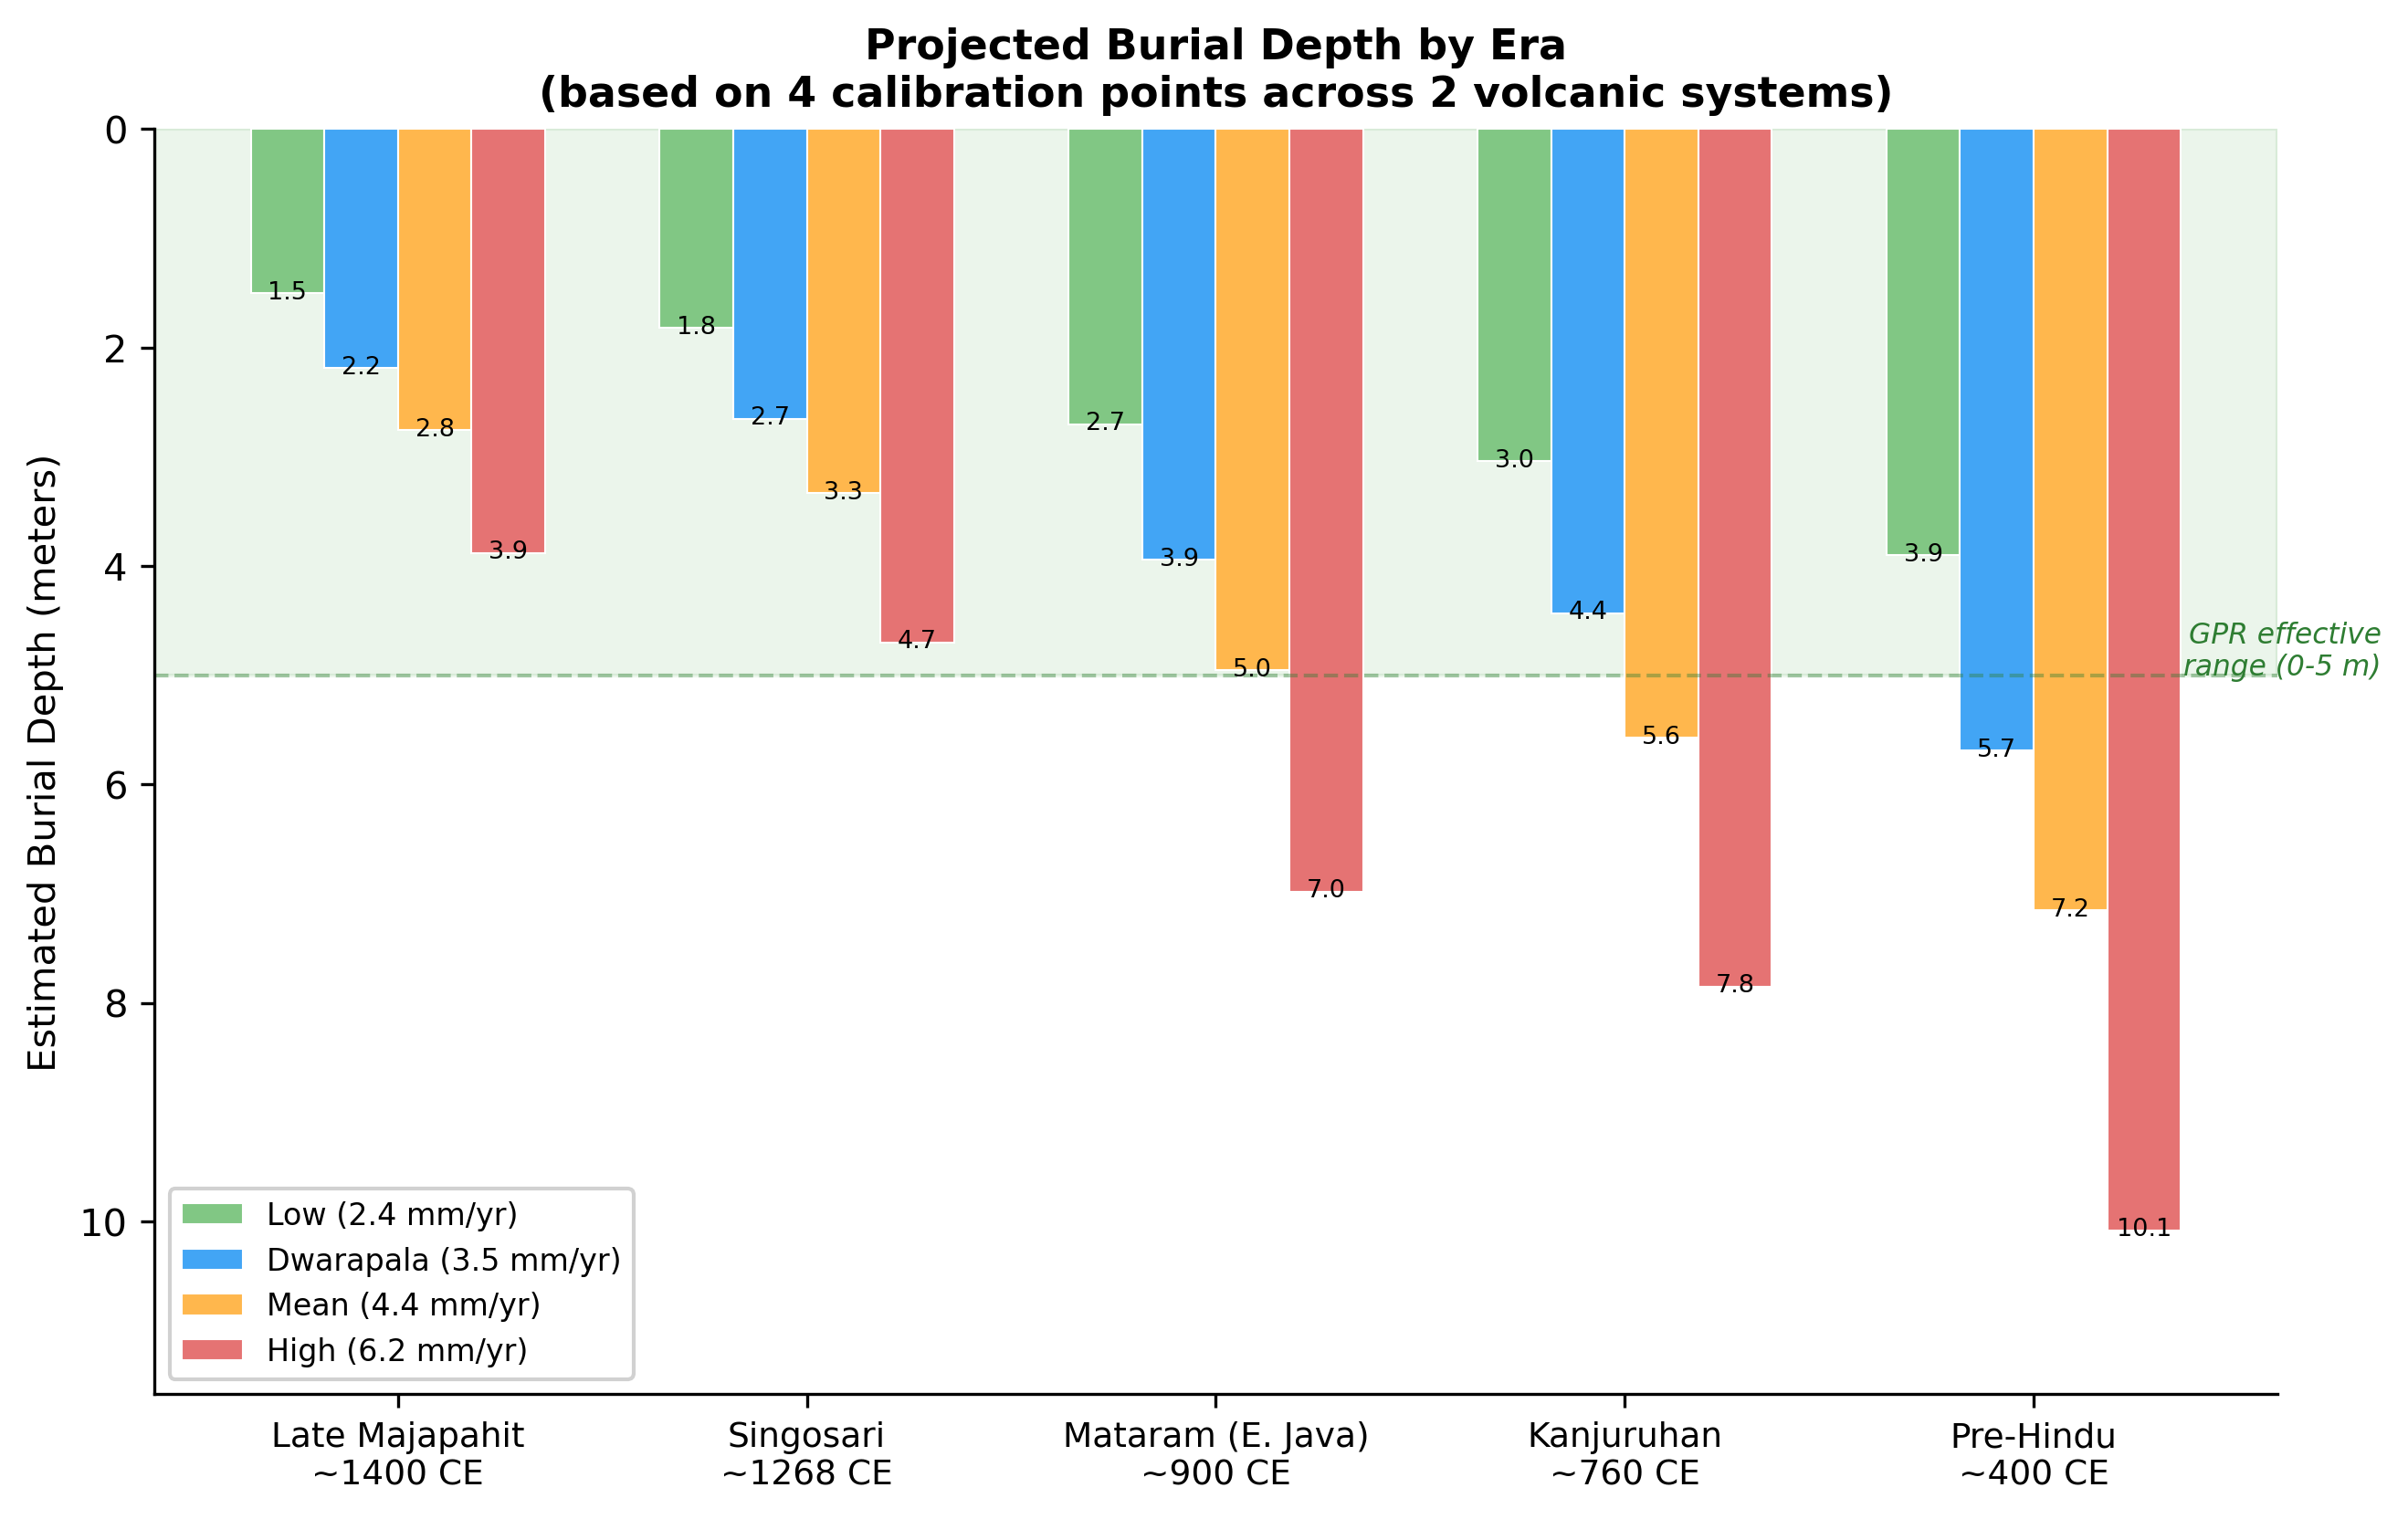
\includegraphics[width=12cm]{figures/fig2_burial_depth_projections.png}
\caption{Projected burial depth by historical era using four empirically-derived sedimentation rates. The green band indicates the effective range of ground-penetrating radar in volcanic sediment (0--5~m). Kanjuruhan-era and earlier remains may exceed GPR detection limits.}
\label{fig:depth}
\end{figure*}

\subsection{Spatial analysis methods}

\textbf{E004---Raw site density vs volcanic proximity.} We computed the minimum great-circle distance from each geocoded site to the nearest of seven reference volcanoes. Sites were binned into seven distance bands (0--25, 25--50, 50--75, 75--100, 100--150, 150--200, and 200+~km). Site density was expressed as sites per 1,000~km\textsuperscript{2}. Spearman's rank correlation between distance band midpoint and site density tests whether sites are found preferentially near or far from volcanoes.

\textbf{E005---Terrain-controlled analysis.} To separate the effect of terrain suitability from volcanic proximity, we constructed a terrain suitability index combining four DEM-derived features (slope, elevation, TWI, and a river proximity proxy). The study area was divided into a 25~km $\times$ 25~km grid (187 cells). For each cell, we computed the residual between observed and terrain-predicted site count. Spearman correlation between residual density and distance to nearest volcano tests the taphonomic bias hypothesis after controlling for terrain preference.


\section{Results}

\subsection{The Dwarapala calibration}

The Dwarapala sedimentation calculation yields a rate of 3.5~mm/year (Sect.~3.2). This rate is internally consistent with documented Kelud eruption histories, which account for approximately 100 of the 185~cm total burial through direct tephra deposition alone. The remaining 85~cm is attributable to secondary remobilization and contributions from other volcanic systems.

The secondary calibration points yield rates of 2.4--6.2~mm/yr across the Merapi system, consistently higher than the Dwarapala rate (3.5~mm/yr) from the Kelud system. This difference is physically plausible: Merapi erupts more frequently than Kelud, and the Central Java sites are closer to their volcanic source. The cross-system mean of $4.4 \pm 1.2$~mm/yr establishes that ongoing volcanic burial is a Java-wide phenomenon with quantifiable, consistent rates.

\subsection{Independent validation}

The 51-pair eruption--site correlation dataset provides a check independent of the four primary calibration sites. Of the 51 pairs, 24 include physically measured burial depths. The mean is 3.41~m (median 2.50~m). Applying the mean calibration rate of 4.4~mm/yr over 760 years (the midpoint historical horizon) predicts 3.3~m. The independent dataset and the calibration model agree within 3\%. This is consistent with---not proof of---the calibration rates representing a true regional baseline rather than a monument-specific artefact.

\subsection{Burial depth projections}

Key projections for the Malang basin using the full rate range:

\begin{table}[t]
\caption{Projected burial depth by era using empirically-derived sedimentation rates.}
\label{tab:depth}
\begin{tabular}{lcccccc}
\tophline
Era & Date (CE) & Elapsed (yr) & Low (2.4) & Dwarapala (3.5) & Mean (4.4) & High (6.2) \\
\middlehline
Late Majapahit & \textasciitilde1400 & 626 & 1.5~m & 2.2~m & 2.8~m & 3.9~m \\
Singosari & \textasciitilde1268 & 758 & 1.8~m & 2.7~m & 3.3~m & 4.7~m \\
Mataram (E. Java) & \textasciitilde900 & 1,126 & 2.7~m & 3.9~m & 5.0~m & 7.0~m \\
Kanjuruhan & \textasciitilde760 & 1,266 & 3.0~m & 4.4~m & 5.6~m & 7.9~m \\
Pre-Hindu & \textasciitilde400 & 1,626 & 3.9~m & 5.7~m & 7.2~m & 10.1~m \\
\bottomhline
\end{tabular}
\belowtable{}
\end{table}

These depths exceed standard archaeological surface survey capabilities (0--1~m) and approach or exceed the effective range of ground-penetrating radar (2--5~m in volcanic sediment) \citep{conyers2004,goodman2013}. Detection of Kanjuruhan-era or earlier remains will likely require deep GPR, borehole coring, or fortuitous exposure through modern construction.

\subsection{Cautionary analysis: why distribution data cannot test the hypothesis}

We conducted two spatial analyses to examine whether the distribution of known sites reflects taphonomic bias. In E004, analysis of 383 geocoded sites revealed a strong \textit{negative} correlation between site density and distance from the nearest active volcano (Spearman's $\rho = -0.955$, $p = 0.0008$, $n = 7$ distance bands; Table~\ref{tab:density}, Fig.~\ref{fig:density}). Known sites cluster \textit{near} volcanoes---the opposite of what a naive reading of the taphonomic bias hypothesis would predict.

\begin{table}[t]
\caption{Site density by distance to nearest active volcano.}
\label{tab:density}
\begin{tabular}{lccc}
\tophline
Distance Band (km) & Sites & Area (km\textsuperscript{2}) & Density (/1,000~km\textsuperscript{2}) \\
\middlehline
0--25 & 147 & 11,343 & 12.96 \\
25--50 & 136 & 18,034 & 7.54 \\
50--75 & 37 & 18,528 & 2.00 \\
75--100 & 22 & 16,373 & 1.34 \\
100--150 & 41 & 28,523 & 1.44 \\
150--200 & 0 & 25,507 & 0.00 \\
200+ & 0 & 73,740 & 0.00 \\
\bottomhline
\end{tabular}
\belowtable{}
\end{table}

\begin{figure*}[t]
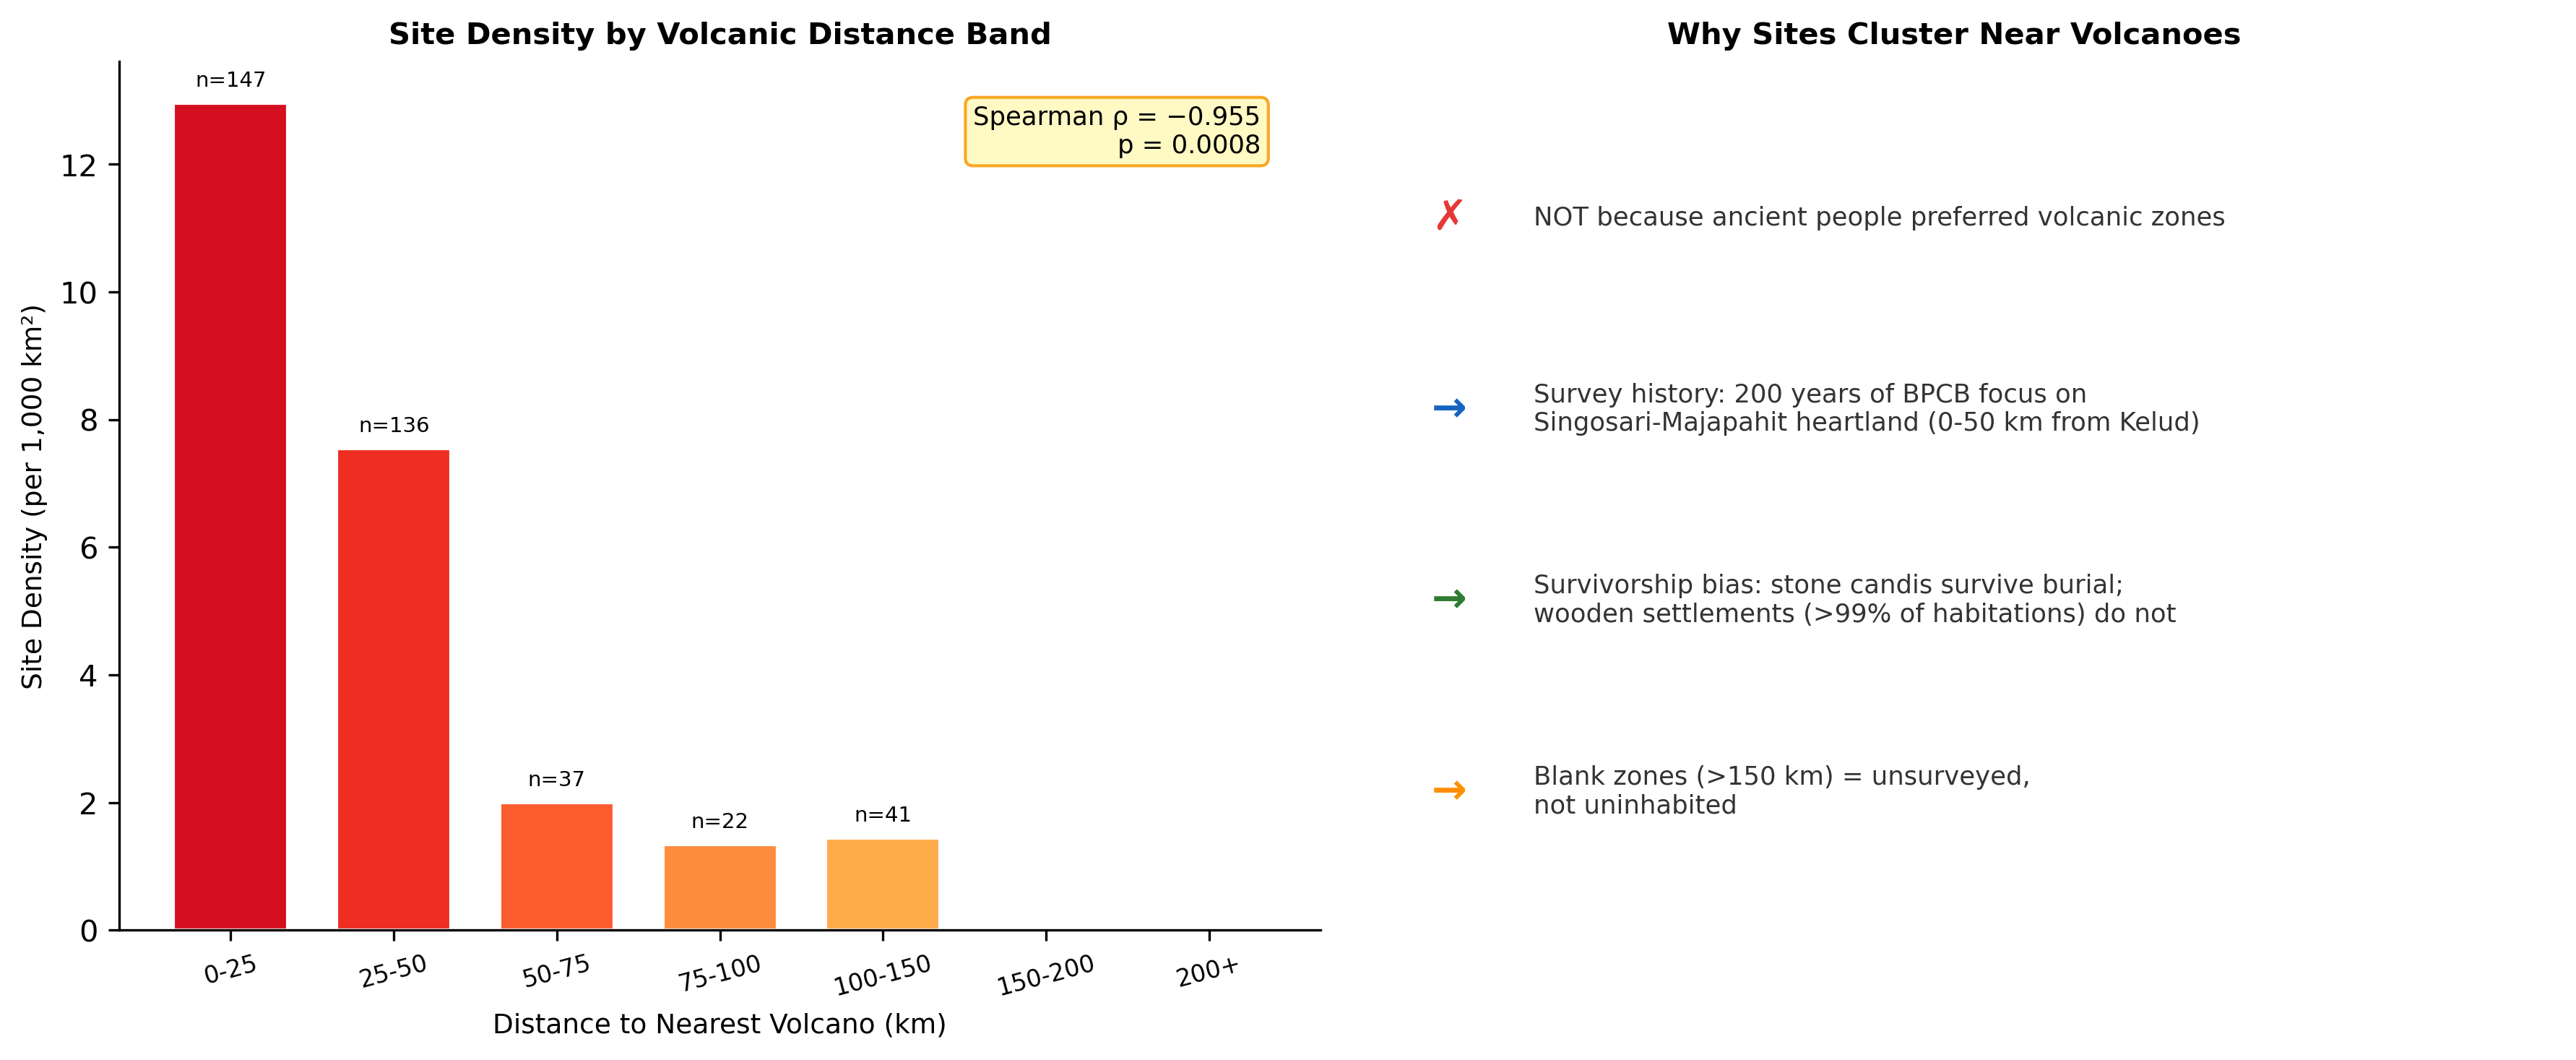
\includegraphics[width=12cm]{figures/fig4_density_vs_distance.png}
\caption{Left: Site density by volcanic distance band showing strong near-volcano clustering ($\rho = -0.955$). Right: Interpretive framework explaining why this pattern reflects survey history, not settlement preference.}
\label{fig:density}
\end{figure*}

In E005, a terrain-controlled analysis using a composite terrain suitability index (slope, elevation, TWI, river proximity) across 187 grid cells of 25~km $\times$ 25~km yielded Spearman's $\rho = -0.358$ ($p < 0.0001$). Terrain suitability explains part of the clustering, but the remaining signal reflects survey intensity concentrated on the Singosari-Majapahit heartland. Repeating both analyses after geocoding 94 additional sites (E006; increasing from 297 to 391 geocoded entries) produced negligible change: E004~$\rho$ shifted from $-0.991$ to $-0.955$; E005~$\rho$ from $-0.364$ to $-0.358$. The pattern is robust.

Critically, these results do \textit{not} test the taphonomic bias hypothesis. The fundamental limitation is circular: the sites in our dataset are those that \textit{survived} burial and were \textit{discovered} by archaeologists. Both processes systematically favor low-burial-depth locations:

\begin{enumerate}
  \item \textbf{Survivorship bias:} Stone temples dominate the dataset because they are large enough to protrude through meters of sediment. Wooden and bamboo structures---$>$99\% of historical habitation---leave no surface trace after burial.
  \item \textbf{Survey bias:} Indonesian archaeological survey has concentrated on regions of known historical kingdoms for over two centuries. ``Blank'' areas on the archaeological map are blank because they are unsurveyed, not uninhabited.
  \item \textbf{Discovery mechanism bias:} Most deeply buried temples were found accidentally during modern construction (Sambisari: farmer's plow, 1966; Kimpulan: university excavation, 2009; Liangan: sand mining, 2008) \citep{putra2019,abbas2016}.
\end{enumerate}

The taphonomic bias hypothesis therefore cannot be confirmed or denied from distribution data alone. It remains a hypothesis requiring subsurface investigation to test. What distribution data \textit{can} establish is the null case: the ``archaeological absence'' of pre-Majapahit evidence in volcanic zones cannot be interpreted as evidence of cultural absence.


\section{Discussion}

\subsection{What 4.4~mm/yr means}

The number that matters is $4.4 \pm 1.2$~mm/yr. Four sites, two volcanic systems, 350~km of separation between the easternmost and westernmost calibration points. They agree within a factor of two. For a process as variable as volcanic sedimentation---driven by eruption frequency, vent distance, wind direction, topography---that agreement is not obvious. It is the finding.

The Kelud-system rate (Dwarapala, 3.5~mm/yr) is slightly lower than the Merapi-system sites (mean \textasciitilde4.8~mm/yr), which is physically reasonable: Merapi erupts more frequently. But both systems produce the same order-of-magnitude result. This is not a Merapi problem or a Kelud problem. It is a Java problem.

\subsection{Why more sites near volcanoes is the expected result}

The spatial analysis produces a result that looks, at first glance, like a refutation of the hypothesis: known sites cluster \textit{near} volcanoes, not away from them ($\rho = -0.955$). But this is exactly what the taphonomic framework predicts, once you account for how the dataset was built.

The 666 sites in our database are not a random sample of all past sites. They are the sites that happened to be large enough to stick out of the ground and located in places where archaeologists have spent the most time. The Singosari-Majapahit heartland near Malang and Mojokerto has been surveyed intensively since Dutch colonial times. It is also where Kelud and Arjuno-Welirang deposit the most ash. So we find sites there because archaeologists looked there, and those particular sites survived because they are massive stone monuments. When we added 94 more geocoded sites from additional sources, the spatial correlation shifted by only 0.036. The database appears to be saturated---not by the actual distribution of past habitation, but by the limits of where people have bothered to look.

\subsection{Practical implications for fieldwork}

The burial depth numbers translate directly into survey recommendations that differ significantly from standard practice in Indonesian archaeology:

\begin{itemize}
  \item \textbf{GPR applicability:} Ground-penetrating radar is effective to \textasciitilde2--5~m in volcanic ash. Late Majapahit-era remains (1.5--3.9~m) are detectable; Kanjuruhan-era remains (3.0--7.9~m) may exceed GPR range \citep{conyers2004}.
  \item \textbf{Priority zones:} Areas with high terrain suitability AND high expected burial depth are where settlement remains are most likely preserved yet invisible.
  \item \textbf{Discovery mechanism:} Accidental discoveries during construction illustrate that deeply buried sites exist but systematic subsurface survey has never been conducted.
\end{itemize}

\subsection{The Kutai comparison}

At 4.4~mm/yr, a Kutai-era (\textasciitilde400~CE) artifact in the Malang basin would now lie beneath 7~m of overburden. The same artifact in Kalimantan (zero volcanism) sits at the original ground surface. The perceived chronological primacy of Kutai over Javanese polities of similar antiquity may reflect this differential preservation, not genuine temporal precedence \citep{coedes1968}.

\subsection{A multiplicative visibility cascade: reframing the primary constraint}

Volcanic burial is not the primary reason early Javanese sites are invisible. Survey coverage is. This is uncomfortable to state in a paper about volcanic burial, but a five-factor visibility model makes it unavoidable:

\begin{equation}
  P(\text{visible}) = P(\text{not buried}) \times P(\text{organic survival}) \times P(\text{surveyed}) \times P(\text{recognized}) \times P(\text{published})
\end{equation}

We stress that these are order-of-magnitude estimates, not precise measurements. Volcanic burial survival ($P \approx 0.58$) derives from our four-site calibration; organic material survival ($P \approx 0.20$) from tropical decomposition literature and the observation that 63\% of inscription-mentioned materials are perishable organics; survey coverage ($P \approx 0.025$) from the ratio of systematically surveyed area to total habitable land; recognition probability ($P \approx 0.40$) and publication probability ($P \approx 0.50$) from professional judgment informed by the colonial-era reporting record. Each factor carries substantial uncertainty. But their product---$0.058\%$ predicted visibility---falls within a factor of two of the observed rate ($0.031\%$, based on 3 ambiguous pre-400~CE sites against \textasciitilde9,600 settlements expected from demographic modeling). The agreement may be partly fortuitous, but the framework identifies which factors matter most.

Survey coverage is the bottleneck: improving it alone would multiply observable sites by 40-fold. Volcanic burial contributes a leverage ratio of 1.7-fold on its own---the smallest of the five factors. But it is the \textit{only} factor that is spatially predictable. We cannot map where organic materials have decayed, or where survey effort was insufficient, or where pre-Hindu sites were misidentified by colonial-era researchers. We \textit{can} map where volcanic burial is deepest. That is the practical value of the calibration framework: not that burial explains everything, but that it tells us exactly where to look.

A separate regression analysis corroborates this picture from a different angle. After controlling for three independent survey intensity proxies---road accessibility, distance to BPCB heritage conservation offices, and distance to university archaeology departments---volcanic proximity remained a significant negative predictor of site density (quasi-Poisson likelihood ratio test: $\beta = -0.477$, $p = 0.0015$, correcting for overdispersion $\phi = 3.55$, $n = 703$ grid cells). The volcanic site deficit is not reducible to differential survey effort; a residual burial signal persists.

A note on what this paper does not claim. One might expect volcanic burial to leave a signature in site-type distributions---destroying open-air sites and leaving only caves and rockshelters, which are harder to bury. Comparative analysis of 80 Island Southeast Asian sites across volcanic and non-volcanic regions finds no such difference (Fisher exact $p = 0.760$). Cave dominance is driven by karst availability, not volcanic burial. This paper does not argue that volcanic burial shifts site-type ratios. The taphonomic framework presented here rests entirely on burial depth measurements: 32 burial-depth measurements compiled from Dutch colonial-era excavation reports \citep{ov1925}, averaging 2.88~m, a sedimentation model validated at $r = 0.951$ against observed depths, and the 51-pair eruption--site correlation dataset. The depth argument is stronger for having the site-type argument stripped away.

\subsection{Limitations}

\begin{enumerate}
  \item \textbf{Calibration sample size:} Four points, while spanning two volcanic systems, remain a small sample. Rates carry uncertainty from imprecise construction dates and variable depth measurements.
  \item \textbf{Monument vs.~settlement calibration:} All four primary calibration points are stone monuments, not open habitation sites. Vertical structures may trap sediment preferentially. However, the independent eruption--site correlation dataset---51 pairs across 12 volcanic systems, including non-monumental contexts---yields a mean burial depth of 3.41~m consistent with the four-point calibration. Monument-derived and settlement-derived rates appear comparable at multi-century timescales.
  \item \textbf{Rate constancy:} We treat sedimentation as temporally uniform, smoothing over episodic large eruptions. This is a deliberate modeling choice, not an unrecognized assumption. The Dwarapala rate averages over \textasciitilde535 years; the Merapi-system rates average over 1,100--1,200 years. Multi-century averaging inherently incorporates multiple eruptive cycles of varying intensity. The wide projection range (2.4--6.2~mm/yr) partially captures inter-site variability arising from different eruption histories.
  \item \textbf{Depth measurement uncertainty:} Published depths vary across sources (e.g., Sambisari: ``5~m'' to ``6.5~m''). We report ranges rather than point estimates.
  \item \textbf{Spatial extrapolation:} Rates derive from two specific volcanic basins. Extrapolation to other Java regions requires additional calibration.
  \item \textbf{Survey bias unquantified:} We argue that survey history dominates distribution data but cannot quantify this without systematic coverage maps.
\end{enumerate}

\subsection{Where this leads}

Knowing burial depths is only useful if it produces fieldwork. The direct next step is a machine learning settlement suitability model that identifies, independently of the burial depth framework, which areas of East Java would have been most attractive to pre-Hindu settlement (Amien, in preparation). Overlaying high suitability with deep predicted burial produces a short list of priority zones---places where evidence is most likely to exist and least likely to have been found. That list is the input for targeted GPR survey and deep coring. The buried sites at Sambisari and Kimpulan were found by accident. The next ones should be found on purpose.


\conclusions

Four calibration points. Two volcanic systems. Three hundred and fifty kilometers between the easternmost and westernmost sites. The sedimentation rates converge at 2.4--6.2~mm/yr, with a mean of $4.4 \pm 1.2$~mm/yr. Four points is a small sample, and we are cautious about generalizing beyond the Kelud and Merapi basins. But the consistency across such different volcanic settings suggests that ongoing burial operates at a regional scale, not as a site-specific anomaly.

The numbers translate directly into what is and is not findable. Kanjuruhan-era remains (\textasciitilde760~CE) in the Malang basin now lie at 3.0--7.9~m depth. Pre-Hindu remains (\textasciitilde400~CE) lie at 3.9--10.1~m. Both ranges exceed conventional surface survey capability and approach the upper limit of ground-penetrating radar. This does not prove that early Javanese settlements exist at these depths. It establishes that we have never systematically looked where they would be.

The spatial analysis adds a sharper constraint. The East Java site record does not map where people lived; it maps where archaeologists have worked and what survived burial by virtue of sheer mass. Stone temples protrude through volcanic sediment because they weigh thousands of tonnes. Wooden settlements do not protrude. The clustering of known sites around the Majapahit--Singosari heartland is an artifact of survey effort, not evidence of cultural absence from volcanic zones.

The oldest conventionally recognized Indonesian kingdom, Kutai, was found at the modern ground surface in Kalimantan, which has no volcanoes. Whether that is a coincidence or a consequence of differential preservation is, we believe, a question that deserves systematic subsurface investigation rather than continued reliance on surface survey alone.


\codedataavailability{The archaeological site dataset, DEM derivatives, and analysis scripts are available at \url{https://github.com/neimasilk/volcarch-repo} (to be made public upon acceptance). Raw DEM data from Copernicus GLO-30 are publicly available. A preprint of this manuscript is available at \url{https://doi.org/10.5281/zenodo.19081502}.}


\authorcontribution{Conceptualization, M.A.; methodology, M.A. and G.F.G.; software, M.A. and G.F.G.; validation, M.A.; formal analysis, M.A.; investigation, M.A.; data curation, M.A.; writing---original draft, M.A.; writing---review and editing, M.A. and G.F.G.; visualization, M.A.}

\competinginterests{The authors declare no competing interests.}

\begin{acknowledgements}
The authors thank the Global Volcanism Program (Smithsonian Institution) for open eruption data, and the OpenStreetMap and Wikidata communities for structured geospatial data.

\textit{AI assistance disclosure.} This research used AI language tools (Claude, Anthropic) for three tasks: systematic screening of historical, epigraphic, and volcanological literature; iterative design and execution of computational experiments; and manuscript drafting and revision. Research design, hypothesis formation, data selection, interpretation, and all conclusions are solely the authors' intellectual contribution. The authors take full responsibility for all claims made in this paper.
\end{acknowledgements}


\bibliographystyle{copernicus}
\bibliography{references}

\end{document}
